\section{Konzept zur Umsetzung der Mitarbeiteransicht}

\subsection{Architekturdesign}
Die Architektur in Next.js ist modular aufgebaut und verwendet wiederverwendbare Komponenten. Jede Komponente ist für einen spezifischen Bereich der Benutzeroberfläche zuständig, wie beispielsweise Header, Footer, Sidebar, Buchungsliste oder Filtermenüs. Dieser Ansatz ermöglicht eine bessere Organisation des Codes, erleichtert die Wartung und reduziert die Wahrscheinlichkeit von Fehlern. Durch die Trennung von Logik und Darstellung innerhalb jeder Komponente können Entwickler Änderungen schneller und sicherer vornehmen.\textit{\cite{rathinam2022analysis}}

\subsection{Datenfluss}
Die Kommunikation zwischen Frontend und Backend wird durch eine REST-API realisiert. Spring Boot, als Backend-Framework, bietet dabei eine native Unterstützung für die Erstellung und Verwaltung von RESTful Webservices. Dies ermöglicht eine flexible Datenübertragung und sorgt für eine klare Trennung zwischen Datenmanagement und Präsentationslogik. Mit dieser Architektur können beispielsweise Buchungsdaten effizient zwischen Frontend und Backend ausgetauscht und verarbeitet werden. \textit{\cite{shetty2020review, rathinam2022analysis}}

\subsection{Prototyping}

Mockups und interaktive Prototypen sind unverzichtbare Schritte im Entwicklungsprozess, um sicherzustellen, dass die geplante Anwendung den Anforderungen und Erwartungen der Nutzer entspricht. Sie legen den Grundstein für eine erfolgreiche Umsetzung und minimieren das Risiko von Fehlentwicklungen.


\subsubsection{Mockups}
Mockups dienen dazu, das endgültige Design vor der Entwicklung zu präsentieren. Sie ermöglichen Feedback und Freigaben, bevor Arbeit in die eigentliche Programmierung investiert wird. Die detaillierte Visualisierung hilft, Missverständnisse zwischen Designern, Entwicklern und Stakeholdern zu minimieren.

Programme wie Sketch, Figma oder Adobe XD werden häufig verwendet, um Mockups zu erstellen. Diese Tools bieten intuitive Funktionen, um präzise Designs zu erstellen und Designideen klar zu kommunizieren.

\newpage

\subsubsection{Interaktive Prototypen}
Der primäre Zweck interaktiver Prototypen liegt in der Durchführung von Usability-Tests, bei denen das Benutzerverhalten analysiert wird. Durch iteratives Feedback können Verbesserungen vorgenommen werden, bevor die eigentliche Entwicklung beginnt.
Programme wie InVision, Figma oder Axure RP ermöglichen die Erstellung von Prototypen mit realistischen Interaktionen.

\begin{figure}
	\centering
	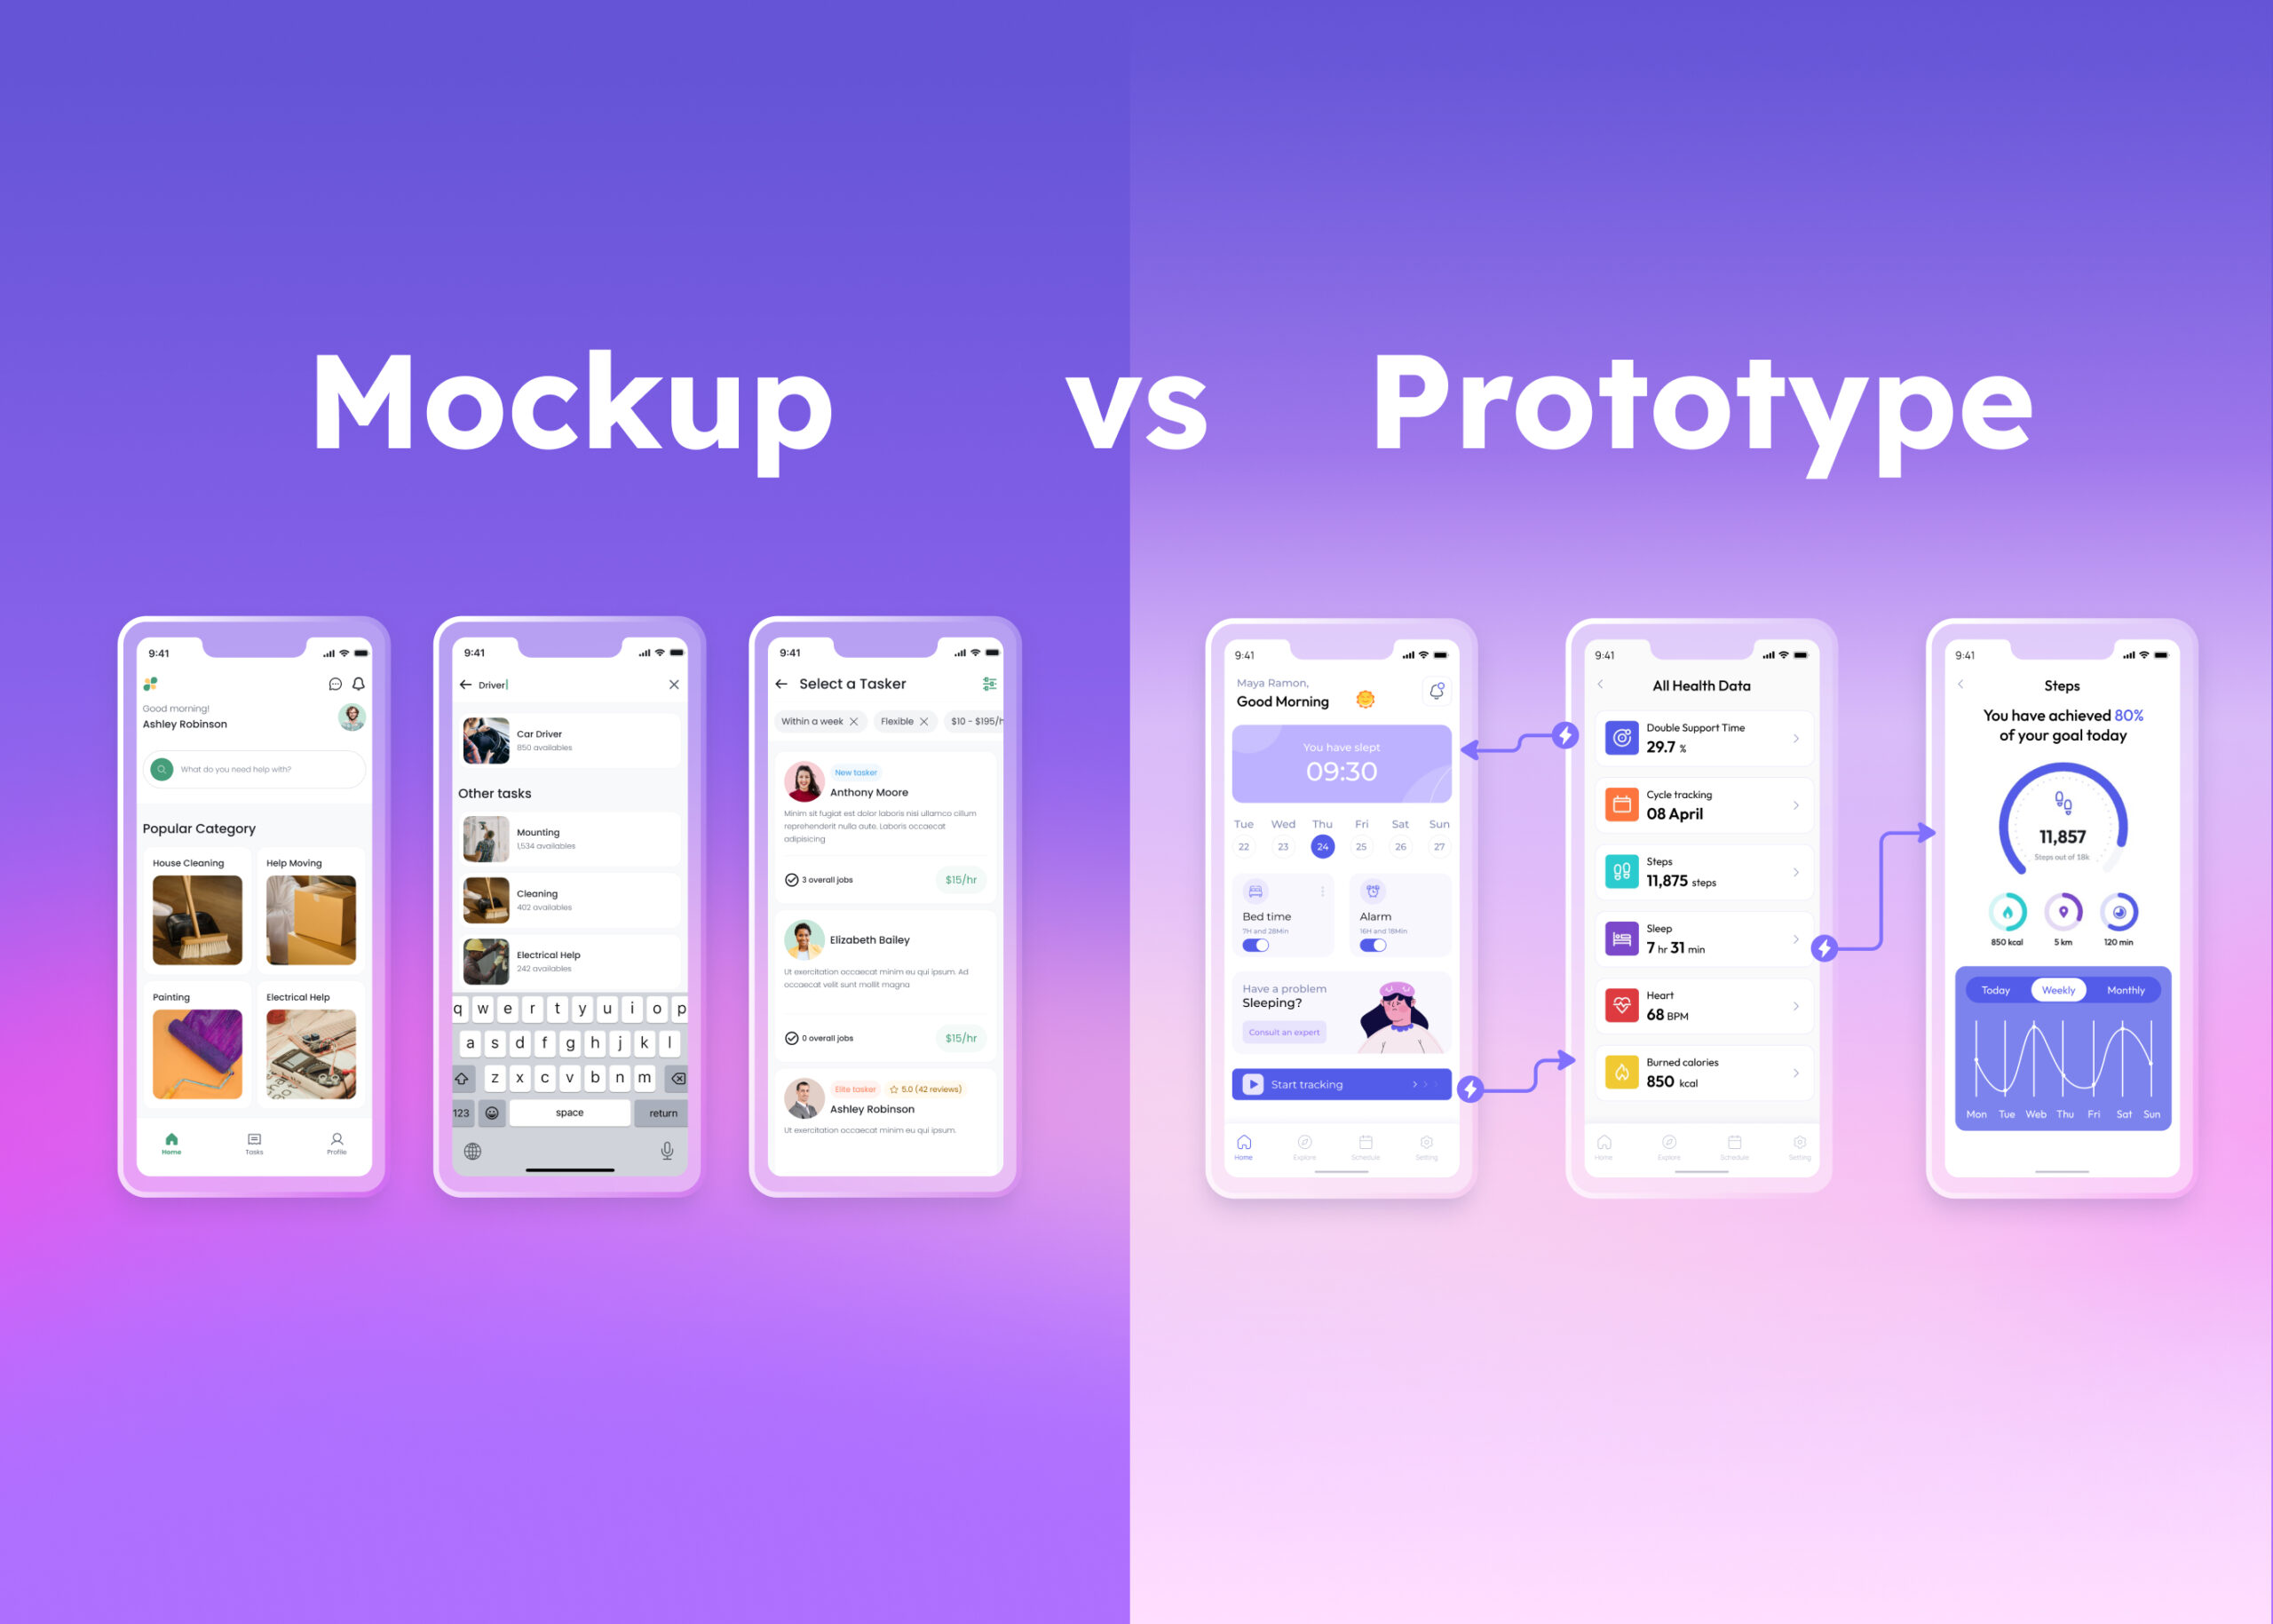
\includegraphics[width=0.75\textwidth]{images/Mockup-vs-Prototype.jpg}
	\caption{Mockup vs Prototype \textit{\cite{mockup_vs_prototype_image}}}
\end{figure}

\newpage

\subsection{Benutzeroberfläche (UI)}

\subsubsection{Struktur der Mitarbeiteransicht}

\textbf{Layout}
\begin{itemize}
	\item \textbf{Widget-basierte Darstellung:} Das Design bietet eine widget-basierte Darstellung, bei der wichtige Informationen in separaten, verschiebbaren und anpassbaren Widgets angezeigt werden. Dies ermöglicht eine flexible und personalisierte Nutzung der Benutzeroberfläche.
	\item \textbf{Responsive Design:} Das Layout passt sich automatisch verschiedenen Bildschirmgrößen an, um eine optimale Benutzererfahrung auf allen Geräten zu gewährleisten (z. B. Desktop, Tablet, Smartphone).
	
	\begin{figure}
		\centering
		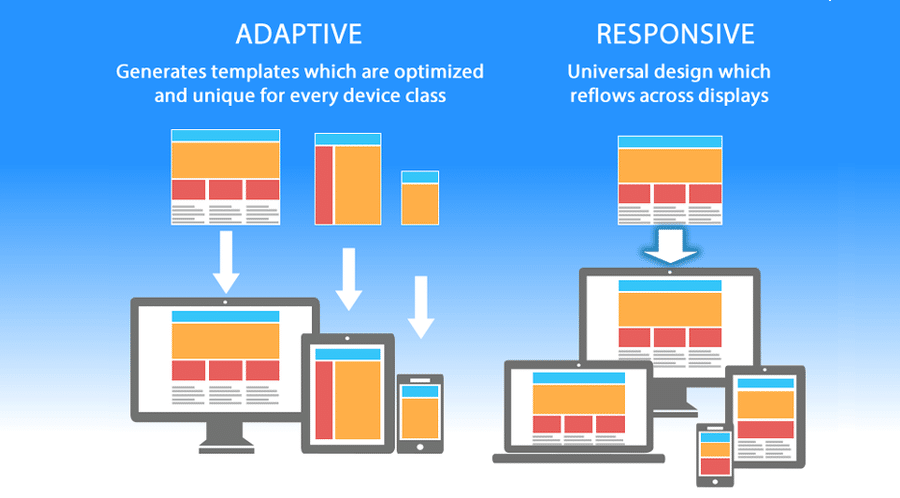
\includegraphics[width=0.75\textwidth]{images/responsive-vs-adaptive.png}
		\caption{Adaptives und responsives Layout\textit{\cite{responsive_vs_adaptive_image}}}
	\end{figure}
\end{itemize}


\subsubsection{Designprinzipien}

\textbf{Konsistenz}
\begin{itemize}
	\item \textbf{Einheitliche Farbpalette:} Primärfarben der Marke, unterstützt durch kontrastierende Akzentfarben. \textit{\cite{ux_usability}}
	\item \textbf{Schriftarten und UI-Komponenten:} Einheitliche Buttons, Dropdown-Menüs und Tooltip-Designs \textit{\cite{ux_usability}}
\end{itemize}

\textbf{Intuitive Bedienung}
\begin{itemize}
	\item \textbf{Eindeutige Beschriftungen:} Aktionen und Felder klar und prägnant benennen.
	\item \textbf{Kontextabhängige Tooltips:} Erklären Funktionen, ohne die Ansicht zu überladen.
	\item \textbf{Progressive Offenlegung:} Fortgeschrittene Optionen erst anzeigen, wenn der Benutzer sie benötigt.
\end{itemize}

\newpage

\subsection{Benutzerfreundlichkeit und Usability}

\textbf{Usability-Tests}
\begin{itemize}
	\item \textbf{Ziel:} Identifikation von Problemen und Ableitung von Verbesserungen für eine optimale Benutzererfahrung. \textit{\cite{ux_usability}}
	\item \textbf{Vorgehen:} 
	\begin{itemize}
		\item Beobachtungen und Analysen erfolgen, um Verbesserungsmöglichkeiten zu identifizieren. \textit{\cite{ux_usability}}
		\item Genutzte Methoden: Think-Aloud, First-Click-Tests und andere explorative Ansätze. \textit{\cite{ux_usability}}
	\end{itemize}
	\item \textbf{Nutzen:} Frühzeitiges Feedback zu Benutzerproblemen und Verbesserung der Benutzerfreundlichkeit. \textit{\cite{ux_usability}}
\end{itemize}


\textbf{Personas und Szenarien}
\begin{itemize}
	\item \textbf{Personas:} Stellt typische Benutzer mit spezifischen Zielen, Bedürfnissen und Herausforderungen dar. Zum Beispiel ein Büroangestellter, der regelmäßig mit Buchungssystemen arbeitet, benötigt intuitive Navigation. \textit{\cite{ux_usability}}
	\item \textbf{Szenarien:} Beschreiben realistische Nutzungssituationen, wie z. B.: „Ein Mitarbeiter möchte eine Buchung ändern und muss dafür die richtige Funktion finden.“ \textit{\cite{ux_usability}}
\end{itemize}

\textbf{Integration in den Entwicklungsprozess}

Durch den Einsatz agiler Methoden können nutzerzentrierte Tests und Feedbackzyklen effizient in den Entwicklungsprozess eingebunden werden. Prototypen und frühe Tests mit Endbenutzern helfen, potenzielle Probleme frühzeitig zu identifizieren und anzupassen.